\chapter{Related Work}
\label{sec:related}

% PointNetVlad, Logg3dNet, EgoNN / ScanContext, STD  / Ransac, ICP, 
% Other papers to cite:
% Handcrafted: SegMap (Dube), M2DP (He)   
% ScanContext modifications: Intesity ScanContext, Semantic ScanContext (SSC) 
% Learned: Locus, Minkloc3d


% Paragraph 1: Overall Introduction
In this section, we first review different LiDAR-based place recognition methods specifically focused on the scenario of place recognition using a single LiDAR scan. Methods involve feature extraction from raw point clouds to retrieve the most similar place and registration of this live point clouds scan to retrieved point clouds to estimate relative transformation. In particular, the second step is important since relative 6-DoF transform between the matches is crucial for integrating loop-closure into a SLAM system. There are various LiDAR-based place recognition approaches exist to extract descriptors: handcrafted models that can extract geometric features and summary statistics \cite{kim2018iros, yuan2023icra}, while learning-based approaches that employ Convolutional Neural Networks (CNNs) to compute high-level descriptors capable of distinguishing between different places \cite{vidanapathirana2022icra, komorowski2022ral}.\vspace{8pt}
 
% \mfallon{also your framing is too narrow - you are talking about systems creating whole scan descriptors. Other methods work by matching segments/clusters.}
% \mfallon{SegMatch is a well cited handcrafted approach. And our own work called NSM (Georgi Tinchev) adapted it to natural environments.}
% \mfallon{SegMap and Georgi's follow up paper extended this approach to use learned descriptors.}
% \mfallon{so I think you should present (a) learned vrs handcrafted; and (b) whole scan vrs cluster based.}
% \haedam{Okay, I try to give an overview. Nived: Can you please check this ?}

% Paragraph 2: Place recognition models, hand crafted 
% ScanContext, Varients, STD
\noindent \textbf{Handcrafted Descriptors:}\hspace{0.5em}  Among handcrafted approaches, ScanContext\cite{kim2018iros,kim2021tro} stands out as a widely adopted technique that generates a descriptor by encoding point clouds in a polar coordinate representation. It captures height information within defined angle and range sectors, then integrates them into a 2D descriptor. 
%The matching of these descriptors enables the estimation of translational and rotational differences between two corresponding point clouds.
ScanContext has also been enhanced by incorporating additional information such as intensity~\cite{wang2020icra} and semantics~\cite{li2021iros} to create more informative descriptors. Another type of handcrafted descriptor, STD~\cite{yuan2023icra}, encodes boundaries of planes as vertices and connects them to create multiple triangles. STD operates without requiring a 360-degree scan, making it compatible with LiDAR systems with only a 90-degree field-of-view (e.g. Livox Aria). Both ScanContext and STD can estimate a relative transformation between corresponding scans by matching their descriptors when detecting loop closure candidates in SLAM or relocalization tasks. However, these existing methods have been primarily tested in urban scenarios. In this work we specifically aim to study their performance in unstructured, natural environments such as forests.
\vspace{8pt}

% \mfallon{you need to unravel this paragraph. it should be 1 ScanContext, 2 extensions of ScanContext and then 3 STD. At the moment it is all rolled together}
% \mfallon{you should cite ScanContext++ - extension by original authors.}
% \mfallon{BTW, the key feature of STD is that it works without needing a 360 scan. For example it works with a Livox Aria 90 degreee lidar.} 
% \haedam{rephrase the order of paragraph. Nived can you check this ?}

% Paragraph 3: Place recognition models, learning based 
\noindent \textbf{Learning-based Descriptors:} \hspace{0.5em} 
Alternatively, recent learning-based models, such as Logg3dNet~\cite{vidanapathirana2022icra}, MinkLoc3D~\cite{komorowski2021wacv}, and EgoNN~\cite{komorowski2022ral} employ discretized representations and contrastive learning schemes to compute point-based local descriptors. This process is followed by generating a global descriptor of aggregated local features using methods like GeM~\cite{radenovic2019pami}, P2O~\cite{vidanapathirana2021icra}, and NetVLAD~\cite{arandjelovic2018pami}.  
% Add P2O high order pooling 

In particular, we are interested in Logg3dNet~\cite{vidanapathirana2022icra} which we primarily tested and integrated into our system. As shown in \figref{fig:logg3dnet}, it uses a sparse convolutional U-network which performs sparse point-voxel convolution on a raw point cloud to embed local features. Local consistency loss (e.g triplet loss) tries to minimize the feature distance between positive pairs (in overlapping locations, typically less than \SI{30}{\meter} apart) while maximizing the feature distance between negative pairs (in non-overlapping locations) in a contrastive manner. These local features are aggregated using second-order pooling followed by differentiable Eigen-value power normalization of SVD to form a global descriptor. A quadruplet loss is used for global descriptors Finally, combined local consistency loss and global scene-level loss are used to train the network in end-to-end fashion. 

Similarly, EgoNN~\cite{komorowski2022ral} employs a deep CNN architecture to extract local descriptors and key points through regression, subsequently aggregating them using GeM to form a global descriptor.
Both EgoNN and Logg3dNet facilitate relative transformation by matching local keypoints with RANSAC, which in turn a final finer resolution registration using ICP. Finally, place recognition models which use Transformers \cite{zhang2019cvpr, xia2021cvpr, zhou2021icra} exist. They are known for their ability to capture long-term dependencies, but have high computational costs and often focus on the global-level place recognition problem not local-level pose estimation. \vspace{8pt}


\begin{figure}
    \centering
    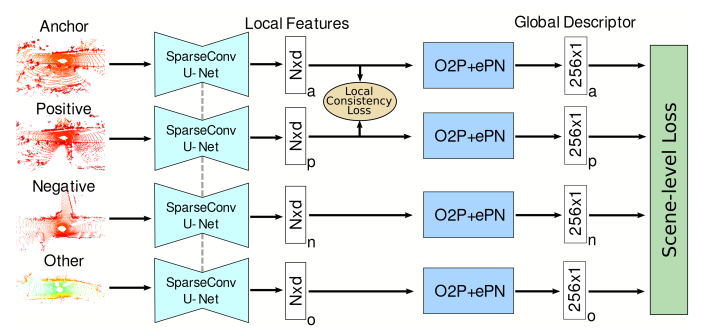
\includegraphics[width=0.7\textwidth]{pics/related_work_logg3dnet_model.png}
    \caption{Logg3dNet architecture. Positive, negative, and anchor point cloud pairs are fed into a SparseConv U-Net with local consistency loss to enforce similarity in local feature embeddings. Local features are aggregated using second-order pooling (O2P) followed by Eigen-value Power Normalization (ePN) to obtain a global descriptor with global scene-level loss. }
    \label{fig:logg3dnet}
\end{figure}
% \mfallon{we need to talk about this - its still too abrupt}
% \mfallon{is the `inability to provide relative pose estimation' inherent in Transformer methods? If not your comment at the end is ill fitting. }
% \haedam{Haedam: Transformer models here only provide global-level place recognition not local-level pose estimation for those cited papers}

% \mfallon{please use `relative transformation' not `relative pose'. Pose is a transformation relative to a fixed coordinate frame (e.g. Odom,.}
% \haedam{Done}
\noindent \textbf{Other types of descriptors:} \hspace{0.5em} 
As an alternative to whole scan descriptors, some methods utilize segments to capture the important elements, effectively compressing the information in the entire point cloud map into a more compact representation. SegMatch \cite{dube2017icra} by Dubé et al. computes local segments and extracts geometric features as a descriptor. In their follow-up work, SegMap \cite{dube2018rss}, these features were learned via a CNN, showing improved overall performance. Tinchev et al. \cite{tinchev2018iros, tinchev2019ral} applied the segment-based approach to natural environments, showing promising results. However, these methods are vulnerable when these segments cannot be reliably detected due to occlusions in dense forest environments, as well as long-term changes in the environment.
\vspace{8pt}

\noindent \textbf{Benchmark datasets:} \hspace{0.5em} 
Several LiDAR point cloud datasets are available for benchmarking place recognition models in urban scenarios \cite{maddern2017ijrr, behley2019iccv, kim2020icra}. However, there are few datasets for natural environments \cite{triest2022icra, knights2023icra}. In particular, the Wild-Places dataset \cite{knights2023icra} is the most notable because it is tailored to large-scale place recognition in forests. This dataset provides point clouds and ground truth poses collected in a forest national park in Australia using hand-held spinning LiDAR at various times of the year. \vspace{8pt}

\noindent In this thesis, we assess the performance of four different place recognition models including both handcrafted (ScanContext and STD) and learning-based (Logg3dNet and EgoNN) models on our dense forest datasets. The datasets contain three different forest environments across different countries, Wytham (UK) which were collected by myself, Evo (Finland) and Stein am Rhein (Switzerland) collected by other member of Oxford Robotics Institute. These datasets were collected using a backpack LiDAR mapping device deep inside the forest, in contrast to previous methods that often concentrated on access roads. 

% The following is the structure of the rest of the thesis. In Chapter 3, we describe overall methods for place recognition and verification with integration of these systems into our SLAM system. In Chapter 4, we describe how this place recognition system was implemented into three different kinds of localization and mapping systems. In Chapter 5, we present the experimental results and analysis of the performance of these models in dense forest environments with different datasets. Finally, in Chapter 6, we conclude the thesis and discuss potential future work.

% These datasets comprise both 32-beam narrow FOV (field-of-view) and 64-beam wide FOV setups . We then integrate these models into our SLAM system and evaluate their performance in identifying robust loop-closure pairs and providing accurate 6-DoF pose estimations within dense forest environments.  Our study focuses on loop-closure capability within dense forest areas, in contrast to previous methods that often concentrated on access roads. 


